\documentclass[notheorems, handout]{beamer}

\usetheme{Warsaw}
\setbeamertemplate{page number in head/foot}[totalframenumber]
\setbeamertemplate{headline}{}
\setbeamertemplate{navigation symbols}{}
\usefonttheme[onlymath]{serif}

\usepackage[utf8]{inputenc}
\usepackage[T2A]{fontenc}
\usepackage[russian]{babel}

\usepackage{graphicx,subcaption,ragged2e}
\usepackage{tikz}
\usepackage{bm}

\newtheorem{remark}{Замечание}

\title[Статистическое и машинное обучение]{Обучение с учителем.
Байесовский подход}
\institute[Санкт-Петербургский Государственный Университет]{%
  \small
  Санкт-Петербургский государственный университет\\
  Кафедра статистического моделирования
}
\date{20 сентября 2025}
\newcommand{\vect}[1]{\mathbf{#1}}
\newcommand{\matr}[1]{\boldsymbol{#1}}
\begin{document}

\begin{frame}
  \titlepage
\end{frame}

\begin{frame}
  \frametitle{Теорема Байеса: ядро подхода}
  \begin{block}{Фундаментальное правило обновления убеждений}
    В байесовском подходе параметры модели $\theta$ рассматриваются
    как случайные величины. Наши знания о них обновляются при
    поступлении данных $D$ с помощью теоремы Байеса.
  \end{block}
  \begin{equation*}
    \underbrace{p(\theta | D)}_{\text{Апостериор}} =
    \frac{\overbrace{p(D | \theta)}^{\text{Ф. правдоподобия}} \cdot
    \overbrace{p(\theta)}^{\text{Априор}}}{\underbrace{p(D)}_{\text{Ф.
    предельного правдоподобия}}} = \frac{p(D | \theta) \cdot
    p(\theta)}{\int{p(D | \theta) \cdot p(\theta) d\theta}}
  \end{equation*}
  \begin{itemize}
    \item \textbf{Априорное распределение $p(\theta)$}: наши
      убеждения о параметрах \textit{до} получения данных.
    \item \textbf{Функция правдоподобия $p(D | \theta)$}: вероятность
      наблюдать данные $D$ при фиксированных параметрах $\theta$.
    \item \textbf{Апостериорное распределение $p(\theta | D)$}:
      обновленные убеждения о $\theta$ \textit{после} учета данных.
  \end{itemize}
\end{frame}

\begin{frame}{Сравнение подходов: частотный и байесовский}
  \textbf{Частотный подход}
  \begin{itemize}
    \item Вероятность --- это долгосрочная частота события.
    \item Параметры модели ($\theta$) --- это фиксированные,
      неизвестные константы.
    \item Результат --- точечные оценки (например, ОМП) и
      доверительные интервалы для $\theta$.
    \item Доверительный интервал (например, 95\%) означает, что при
      многократном повторении эксперимента 95\% таких интервалов
      будут содержать истинное значение параметра.
  \end{itemize}
  \textbf{Байесовский подход}
  \begin{itemize}
    \item Вероятность --- это степень уверенности в утверждении.
    \item Параметры модели ($\theta$) --- это случайные величины с
      распределениями.
    \item Результат --- апостериорное распределение параметров $\theta$.
    \item Доверительный интервал (например, 95\%) означает, что
      существует 95\%-ая вероятность того, что истинное значение
      параметра находится в этом интервале.
  \end{itemize}
\end{frame}
\begin{frame}
  \frametitle{Теорема Бернштейна--фон Мизеса}
  \begin{block}{Теорема Бернштейна--фон Мизеса}
    При определенных условиях регулярности, для больших $N$
    апостериорное распределение $p(\theta|D)$ сходится к нормальному
    распределению:
    $$ p(\theta|D) \approx \mathcal{N}(\theta \mid
    \hat{\theta}_{\text{MLE}}, [E_N(\hat{\theta}_{\text{MLE}})]^{-1}) $$
    \textbf{Следствие:}
    \begin{itemize}
      \item Апостериорное распределение становится гауссианой.
      \item Его центр $\hat{\theta}_{\text{MLE}}$ является
        состоятельной оценкой истинного значения $\theta_0$.
      \item Его дисперсия (неопределенность) уменьшается с ростом $N$.
      \item \textbf{Апостериорное распределение больше не зависит от
        выбора априорного при больших N.}
    \end{itemize}
  \end{block}

\end{frame}
\begin{frame}
  \frametitle{Гибридный  подход к классификации}
  Гибридный подход подразумевает, что мы оцениваем параметры
  правдоподобия (например, среднее и дисперсию для нормального
  распределения) как точные значения из данных.
  \begin{block}{Формальный байесовский подход }
    \begin{enumerate}
      \item \textbf{Моделирование}: Для каждого класса $k$ мы
        оцениваем плотность вероятности признаков $p(\vect{x}|y=k)$ и
        априорную вероятность класса $p(y=k)$.
      \item \textbf{Классификация}: Используем теорему Байеса для
        вычисления апостериорной вероятности:
        $$ p(y=k|\vect{x}) = \frac{p(\vect{x}|y=k) p(y=k)}{p(\vect{x})} $$
        И выбираем класс, который ее максимизирует.
    \end{enumerate}
  \end{block}
\end{frame}
\begin{frame}
  \frametitle{Наивный байесовский классификатор}
  \begin{block}{Ключевое ( ``наивное'') предположение}
    Признаки $\vect{x} = (x_1, x_2, \dots, x_d)$ \textbf{условно
    независимы} при заданном классе $y=k$.
  \end{block}
  Математически это означает:
  $$ p(\vect{x}|y=k) = p(x_1, \dots, x_d|y=k) = \prod_{j=1}^{d} p(x_j|y=k) $$

  Это предположение резко упрощает задачу. Вместо оценки сложной
  многомерной плотности $p(\vect{x}|y=k)$, нам нужно оценить $d$
  одномерных плотностей $p(x_j|y=k)$.

  \begin{block}{Правило классификации}
    $$ \hat{y} = \arg\max_k \left( \log p(y=k) + \sum_{j=1}^{d} \log
    p(x_j|y=k) \right) $$
  \end{block}
\end{frame}

\begin{frame}
  \frametitle{Вариации в зависимости от типа данных}
  Вид классификатора определяется выбором распределения для функции
  правдоподобия $p(x_j|y=k)$.

  \begin{columns}[T]
    \column{0.33\textwidth}
    \begin{block}{Gaussian NB}
      \textbf{Данные}: Непрерывные\\
      \textbf{Модель}: $p(x_j|y=k)$ --- нормальное распределение
      $\mathcal{N}(\mu_{jk}, \sigma_{jk}^2)$\\
      \textbf{Пример}: Классификация ирисов по длине и ширине лепестков
    \end{block}

    \column{0.33\textwidth}
    \begin{block}{Multinomial NB}
      \textbf{Данные}: Дискретные (счетчики)\\
      \textbf{Модель}: $p(x_j|y=k)$ --- мультиномиальное распределение\\
      \textbf{Пример}: Классификация текстов. $x_j$ --- частота
      $j$-го слова в документе
    \end{block}

    \column{0.33\textwidth}
    \begin{block}{Bernoulli NB}
      \textbf{Данные}: Бинарные (0/1)\\
      \textbf{Модель}: $p(x_j|y=k)$ --- распределение Бернулли\\
      \textbf{Пример}: Анализ спама. $x_j=1$, если $j$-е слово есть в
      письме, и $0$ иначе
    \end{block}
  \end{columns}
\end{frame}

\begin{frame}
  \frametitle{LDA и QDA}
  Дискриминантный анализ  решают задачу классификации, моделируя
  распределение данных для каждого класса.
  \begin{block}{Ключевое предположение}
    Плотность распределения признаков для каждого класса $k$ является
    многомерным нормальным распределением:
    $$ p(\vect{x}|y=k) \sim \mathcal{N}(\matr{\mu}_k, \matr{\Sigma}_k) $$
  \end{block}
  Для удобства вычислений переходим к логарифму апостериорной вероятности:
  $$ \hat{y} = \arg\max_k \left( \log p(\vect{x}|y=k) + \log p(y=k) \right) $$
  Подставляя логарифм плотности Гаусса, получаем дискриминантную
  функцию $\delta_k(\vect{x})$:
  $$ \delta_k(\vect{x}) = -\frac{1}{2}\log|\matr{\Sigma}_k| -
  \frac{1}{2}(\vect{x}-\matr{\mu}_k)^T\matr{\Sigma}_k^{-1}(\vect{x}-\matr{\mu}_k)
  + \log \pi_k $$
  где $\pi_k = p(y=k)$ --- априорная вероятность класса.
\end{frame}

\begin{frame}
  \frametitle{Квадратичный дискриминантный анализ (QDA)}
  \begin{block}{Предположение QDA}
    Каждый класс $k$ имеет собственную матрицу ковариаций $\matr{\Sigma}_k$.
  \end{block}

  Дискриминантная функция $\delta_k(\vect{x})$ является квадратичной
  функцией от $\vect{x}$:
  $$ \delta_k(\vect{x}) =
  -\frac{1}{2}\vect{x}^T\matr{\Sigma}_k^{-1}\vect{x} +
  \vect{x}^T\matr{\Sigma}_k^{-1}\matr{\mu}_k -
  \frac{1}{2}\matr{\mu}_k^T\matr{\Sigma}_k^{-1}\matr{\mu}_k
  -\frac{1}{2}\log|\matr{\Sigma}_k| + \log \pi_k $$
  \begin{itemize}
    \item Условие $\delta_k(\vect{x}) = \delta_j(\vect{x})$ задает
      квадратичную разделяющую поверхность (эллипсоид, параболоид, гиперболоид).
    \item QDA --- очень гибкий метод, но требует оценки большого
      числа параметров для каждой матрицы $\matr{\Sigma}_k$, что
      может привести к переобучению на малых выборках.
  \end{itemize}
\end{frame}

\begin{frame}
  \frametitle{Линейный дискриминантный анализ (LDA)}
  \begin{block}{Предположение LDA}
    Все классы имеют общую матрицу ковариаций $\matr{\Sigma}_k = \matr{\Sigma}$.
  \end{block}

  Это упрощение сильно меняет дискриминантную функцию. Член
  $\vect{x}^T\matr{\Sigma}^{-1}\vect{x}$ становится одинаковым для
  всех классов и не влияет на $\arg\max_k$.

  \begin{block}{Линейная дискриминантная функция}
    $$ \delta_k(\vect{x}) = \vect{x}^T\matr{\Sigma}^{-1}\matr{\mu}_k
    - \frac{1}{2}\matr{\mu}_k^T\matr{\Sigma}^{-1}\matr{\mu}_k + \log\pi_k $$
  \end{block}
  \begin{itemize}
    \item Это линейная функция от $\vect{x}$.
    \item Разделяющая поверхность $\delta_k(\vect{x}) =
      \delta_j(\vect{x})$ является гиперплоскостью.
    \item LDA более устойчив к переобучению, чем QDA, так как
      оценивается меньше параметров.
  \end{itemize}
\end{frame}
\begin{frame}
  \frametitle{Визуализация разделяющих поверхностей}
  \begin{figure}
    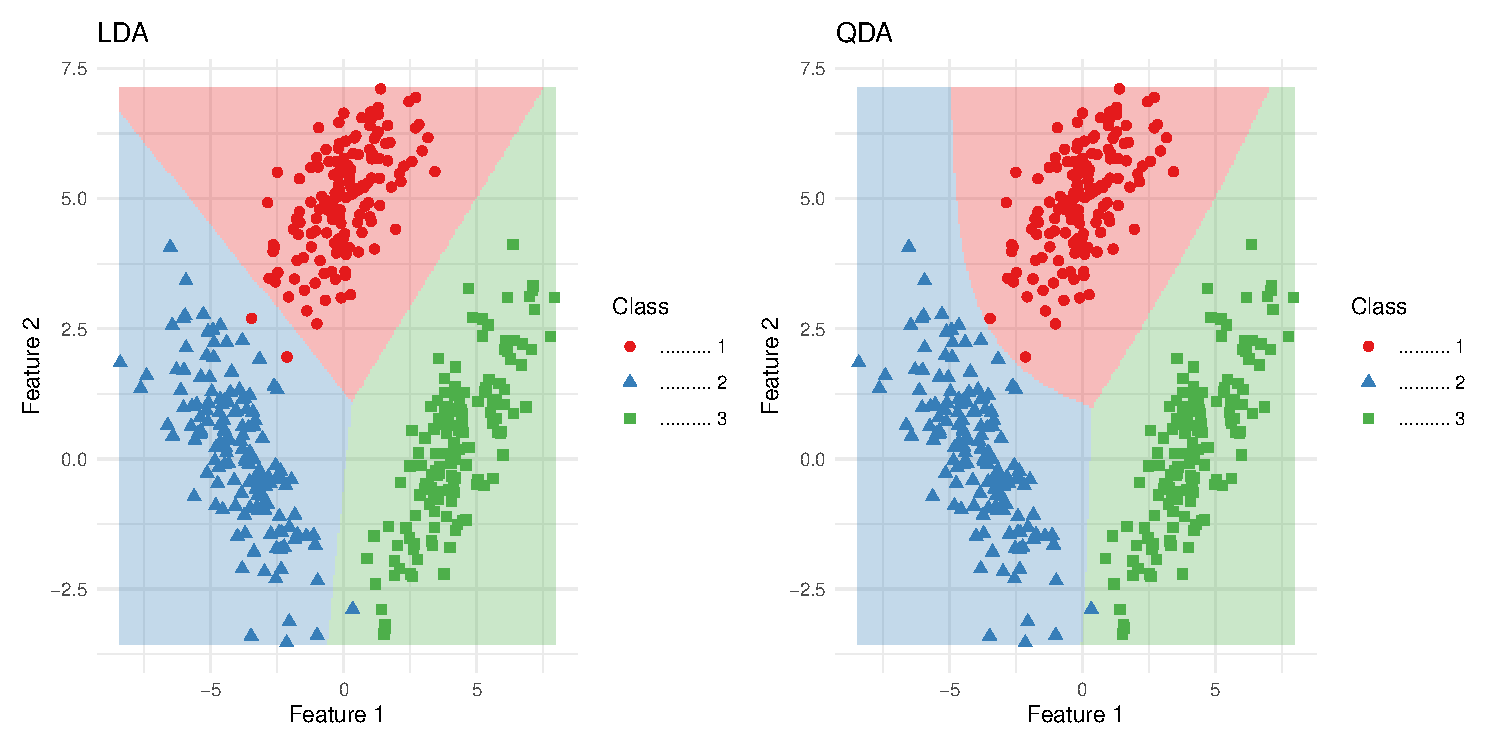
\includegraphics[width=\textwidth]{img/lda_vs_qda.pdf}
    \caption{Слева: LDA создает линейные границы. Справа: QDA создает
      гибкие квадратичные границы, которые лучше разделяют классы с
    разной формой ковариации.}
  \end{figure}
\end{frame}
\begin{frame}
  \frametitle{Байесовское иерархическое моделирование}
  Полностью байесовский (иерархический) подход к классификации
  заключается в том, что мы не уверены не только в классе объекта, но
  и в точных параметрах, описывающих этот класс.\\
  \textbf{Иерархический} аспект таких моделей заключается в том, что
  мы организуем наши параметры на разных
  уровнях.\\ \textbf{Байесовский} аспект заключается в том, что мы
  корректируем наши представления об этих параметрах на основе
  наблюдаемых данных.

  \begin{block}{Структура иерархической модели}
    Параметры модели сами рассматриваются как случайные величины,
    взятые из распределения более высокого уровня.
    \begin{itemize}
      \item \textbf{Уровень 1 (Данные):} $x \sim \text{Распределение}(\theta_k)$
      \item \textbf{Уровень 2 (Параметры классов):} $\theta_k \sim
        \text{Распределение}(\lambda)$
      \item \textbf{Уровень 3 (Гиперпараметры):} $\lambda \sim
        \text{Гиперприор}$
    \end{itemize}
  \end{block}



\end{frame}
\begin{frame}
  \frametitle{Байесовское иерархическое моделирование}
  \begin{block}{Пример: Средние $\mu_{jk}$ в гауссовском наивном Байесе}
    \begin{itemize}
      \item[$\bullet$] Вместо того чтобы считать каждое $\mu_{jk}$
        независимым, мы предполагаем, что все они взяты из общего
        ``материнского'' распределения:
        $$ \mu_{jk} \sim \mathcal{N}(\mu_{j, global}, \sigma^2_{j, global}) $$
      \item[$\bullet$] Модель оценивает и $\mu_{jk}$, и общие
        $\mu_{j, global}, \sigma^2_{j, global}$ одновременно.
    \end{itemize}
  \end{block}
  Оценка для редкого класса становится компромиссом между его
  собственными данными и средним по всем классам. Это делает модель
  гораздо более устойчивой к выбросам.

\end{frame}

\begin{frame}{Байесовская линейная регрессия}
  \textbf{Частотная линейная регрессия:}
  \begin{itemize}
    \item Модель: $y = \vect{w}^T\vect{x} + \epsilon$, где $\epsilon
      \sim N(0, \sigma^2)$.
    \item Цель: найти точечные оценки коэффициентов $\beta$, которые
      минимизируют сумму квадратов ошибок.
    \item Результат: вектор коэффициентов $\hat{\beta}$ и их
      доверительные интервалы.
  \end{itemize}
  \vspace{0.5cm}
  \textbf{Байесовская линейная регрессия:}
  \begin{itemize}
    \item Модель та же, но на параметры $\vect{w}$ и $\sigma^2$
      задаются априорные распределения, например, $\vect{w} \sim N(0,
      \alpha^{-1}I)$.
    \item Цель: найти апостериорные распределения для $\vect{w}$.
    \item Результат: полные распределения для каждого коэффициента,
      которые показывают нашу неуверенность в оценках.
  \end{itemize}
\end{frame}
\begin{frame}
  \frametitle{Математическая модель}
  Предполагаем, что шум аддитивный и гауссовский: $\epsilon \sim
  \mathcal{N}(0, \sigma^2)$.
  Тогда функция правдоподобия для одного объекта $(\vect{x}_i, y_i)$ имеет вид:
  $$ p(y_i|\vect{x}_i, \vect{w}) = \mathcal{N}(y_i |
  \vect{w}^T\vect{x}_i, \sigma^2) $$
  Для всей выборки $D = \{(\vect{x}_i, y_i)\}_{i=1}^N$:
  $p(D|\vect{w}) = \prod_i \mathcal{N}(y_i | \vect{w}^T\vect{x}_i, \sigma^2)$.

  \vspace{1em}
  \textbf{Априорное распределение}

  Чтобы избежать переобучения, вводим априорное распределение на веса
  $\vect{w}$. Обычно используется гауссовское распределение с центром в нуле:
  $$ p(\vect{w}) = \mathcal{N}(\vect{w} | \vect{0}, \alpha^{-1}\matr{E}) $$
  \begin{itemize}
    \item Параметр $\alpha$ контролирует ``разброс'' весов. Большое
      $\alpha$ ``стягивает'' веса к нулю.
    \item Это эквивалентно L2-регуляризации в частотном подходе.
  \end{itemize}
\end{frame}

\begin{frame}
  \frametitle{Связь с L2-регуляризацией}
  $$ \mathbf{w}_{\text{MAP}} = \arg\max_{\mathbf{w}} p(\mathbf{w}|D)
  = \arg\max_{\mathbf{w}} \left( \log p(D|\mathbf{w}) + \log
  p(\mathbf{w}) \right) $$
  \[
    \log p(D|\mathbf{w}) = \log \prod_{i=1}^N
    \mathcal{N}(y_i|\mathbf{w}^T\mathbf{x}_i, \sigma^2) =
    -\frac{1}{2\sigma^2} \sum_{i=1}^N (y_i -
    \mathbf{w}^T\mathbf{x}_i)^2 + \text{const}
  \]
  \begin{multline*}   \log p(\mathbf{w}) = \log
    \mathcal{N}(\mathbf{w}|\mathbf{0}, \alpha^{-1}\mathbf{I})  = \log
    \left( C \cdot
      \exp\left(-\frac{1}{2}\mathbf{w}^T(\alpha^{-1}\mathbf{I})^{-1}\mathbf{w}\right)
    \right) \\
    =  -\frac{\alpha}{2} ||\mathbf{w}||_2^2 + \text{const}
  \end{multline*}
  \begin{align*}
    \mathbf{w}_{\text{MAP}} &= \arg\max_{\mathbf{w}} \left(
      -\frac{1}{2\sigma^2} \sum_{i=1}^N (y_i -
    \mathbf{w}^T\mathbf{x}_i)^2 - \frac{\alpha}{2} ||\mathbf{w}||_2^2 \right) \\
    % Умножаем на 2\sigma^2, что не меняет точку минимума
    &= \arg\min_{\mathbf{w}} \left( \sum_{i=1}^N (y_i -
      \mathbf{w}^T\mathbf{x}_i)^2 + \sigma^2\alpha_{\lambda}
    ||\mathbf{w}||_2^2 \right)
  \end{align*}

\end{frame}

\begin{frame}
  \frametitle{Апостериорное распределение и предсказание}
  \begin{block}{Апостериорное распределение для весов}
    Так как априорное распределение и функция правдоподобия являются
    гауссовскими, то и апостериорное распределение $p(\vect{w}|D)$
    тоже будет гауссовским (свойство сопряженности).
    $$ p(\vect{w}|D) \sim \mathcal{N}(\vect{w} | \vect{m}_N, \matr{S}_N) $$
    где $\vect{m}_N$ и $\matr{S}_N$ вычисляются на основе данных.
  \end{block}

  Для нового объекта $\vect{x}_*$ предсказание $y_*$ --- это не одно
  число, а целое распределение. Оно получается путем усреднения по
  всем возможным весам $\vect{w}$ с учетом их апостериорной вероятности:
  \[ p(y_*|\vect{x}_*, D) = \int p(y_*|\vect{x}_*, \vect{w})
  p(\vect{w}|D) d\vect{w} \]
  Это распределение также является гауссовским. Его среднее --- это
  наше предсказание, а дисперсия --- мера нашей неуверенности в этом
  предсказании.
\end{frame}

\begin{frame}{Вычисление апостериорного распределения}
  Для вычисления апостериорного распределения $p(\theta|D) \propto
  p(D|\theta)p(\theta)$ необходимо вычислить знаменатель (функцию
  предельного правдоподобия):
  \begin{equation*}
    P(D) = \int P(D | \theta) P(\theta) d\theta
  \end{equation*}
  \begin{itemize}
    \item Этот интеграл часто является невычислимым аналитически,
      особенно в моделях с большим числом параметров.
    \item Существует два основных подхода к решению этой проблемы:
      \begin{enumerate}
        \item Аналитический вывод с использованием сопряженных
          априорных распределений.
        \item Численные методы, такие как методы Монте-Карло по схеме
          марковских цепей (MCMC).
      \end{enumerate}
  \end{itemize}
\end{frame}

\begin{frame}{Аналитический подход: Сопряженные распределения}
  \begin{block}{Определение}
    Априорное распределение $P(\theta)$ называется сопряженным для
    функции правдоподобия $P(D|\theta)$, если получаемое
    апостериорное распределение $P(\theta|D)$ принадлежит тому же
    семейству распределений, что и априорное.
  \end{block}
  Вместо сложного интегрирования, весь процесс байесовского
  обновления сводится к простому вычислению новых параметров по
  готовым формулам. Это делает вывод быстрым и аналитически
  разрешимым. Выбор сопряженных пар (Нормальное--Нормальное,
  Бета--Бернулли, Гамма--Пуассона и т.д.) --- это основной способ
  сделать байесовский анализ вычислительно возможным.

\end{frame}

\begin{frame}{Аналитический подход: Сопряженные распределения}
  \textbf{Пример:}
  \begin{itemize}
    \item \textbf{Правдоподобие (Биномиальное):} Моделируем $k$
      успехов в $n$ испытаниях с вероятностью успеха $\theta$.
      \begin{equation*}
        P(D|\theta) = \text{Bin}(k|n, \theta) \propto \theta^k (1-\theta)^{n-k}
      \end{equation*}
    \item \textbf{Априорное (Бета):} Предполагаем, что $\theta$
      следует Бета-распределению.
      \begin{equation*}
        P(\theta) = \text{Beta}(\theta|\alpha, \beta) \propto
        \theta^{\alpha-1} (1-\theta)^{\beta-1}
      \end{equation*}
    \item \textbf{Апостериорное (Бета):} Апостериорное распределение
      также является Бета-распределением.
      \begin{equation*}
        P(\theta|D) \propto \theta^{k+\alpha-1}
        (1-\theta)^{n-k+\beta-1} = \text{Beta}(\theta|k+\alpha, n-k+\beta)
      \end{equation*}
  \end{itemize}
\end{frame}
\begin{frame}{Численный подход: Методы MCMC}
  \begin{itemize}
    \item \textbf{Идея:} Если мы не можем аналитически описать
      апостериорное распределение, мы можем сгенерировать из него выборку.
    \item MCMC (Markov Chain Monte Carlo) --- это алгоритм, строящий
      марковскую цепь, стационарное распределение которой совпадает с
      искомым апостериорным распределением $p(\theta|D)$.
    \item Использование сопряженных априорных распределений удобно,
      но часто является сильным упрощением.
    \item Мы хотим использовать более гибкие или более реалистичные
      априорные распределения, которые не являются сопряженными.
    \item Модель сложна, и найти сопряженное распределение для всех
      параметров невозможно.
  \end{itemize}
  \vspace{0.5cm}
\end{frame}

\begin{frame}{Численный подход: Методы MCMC}
  \textbf{Пример:}
  \begin{enumerate}
    \item Начинаем со случайного значения параметра $\theta_0$.
    \item На каждой итерации $t$:
      \begin{itemize}
        \item Предлагаем нового кандидата $\theta'$ из некоторого
          предложенного распределения $q(\theta'|\theta_{t-1})$.
        \item Вычисляем коэффициент принятия $\alpha =
          \frac{p(\theta'|D)}{p(\theta_{t-1}|D)}$. Так как
          $p(\theta|D) \propto p(D|\theta)p(\theta)$, нам не нужно
          знать нормализующую константу.
        \item Принимаем кандидата ($\theta_t = \theta'$) с
          вероятностью $\min(1, \alpha)$, иначе оставляем старое
          значение ($\theta_t = \theta_{t-1}$).
      \end{itemize}
    \item После достаточного числа итераций полученные значения
      $\{\theta_t\}$ будут выборкой из апостериорного распределения.
  \end{enumerate}
\end{frame}

\end{document}